\section{Deep Q-Networks}
\label{sec:dqn}

The deep Q-network (DQN) demonstrated that Q-learning with
function approximation could work at scale, learning to play
dozens of video games directly from raw pixels at
human-competitive levels~\citep{mnih2015human}. With the neural
network foundations from \cref{sec:deep-learning} in hand, we can
now describe the specific architecture and training techniques
that made this possible. DQN is Q-learning with a convolutional
neural network as the function approximator, plus two techniques
that tame the instability flagged in \cref{subsec:func-approx}:
\emph{experience replay}, which breaks the correlations between
consecutive training samples, and a \emph{target network}, which
stabilizes the learning target. This section describes each
component in turn.

\subsection{Preprocessing}
\label{subsec:preprocessing}

\Cref{sec:deep-learning} introduced the building blocks of neural
networks, including convolutional layers designed for spatial
inputs. Before the network can process a game frame, the raw
output must be transformed into a compact input.

\smallskip
The raw output of a video game environment is a sequence of color
frames -- $210 \times 160$ pixels with three color channels, rendered
at 60 frames per second. Feeding these directly into a neural network
would be wasteful: neighboring frames are nearly identical, color
carries little task-relevant information, and the resolution is
higher than needed. A four-step preprocessing pipeline reduces each
frame to a compact representation before the network sees it.

\smallskip
First, the agent takes the pixelwise maximum of two consecutive raw
frames. Some game environments render certain sprites on alternating
frames -- an object may appear in one frame and vanish in the next
due to hardware limitations in how sprites are drawn. The max
operation ensures that all objects are visible in every processed
frame.

\smallskip
Second, the frame is converted to grayscale by extracting the
luminance channel. For most games, the spatial layout of objects
matters far more than their color, and reducing from three channels
to one cuts the input size by two-thirds.
\Cref{fig:grayscale} illustrates the transformation.

\begin{figure}[ht]
\centering
\begin{tikzpicture}[
    lbl/.style={font=\scriptsize, text=black!55},
    dimlbl/.style={font=\tiny, text=black!45},
    clbl/.style={font=\scriptsize\bfseries},
]
\def\c{0.095}

% --- Helper: draw 21x16 face grid ---
% #1=x-offset, #2=bg (outside face), #3=face fill,
% #4=feature fill, #5=outline fill, #6=draw color
\newcommand{\drawface}[6]{%
    \foreach \x in {0,...,20} {
        \foreach \y in {0,...,15} {
            % Distance from face center (10, 7.5)
            \pgfmathsetmacro{\dist}{sqrt((\x-10)*(\x-10)+(\y-7.5)*(\y-7.5))}
            \pgfmathtruncatemacro{\inface}{\dist < 6.3 ? 1 : 0}
            \pgfmathtruncatemacro{\onedge}{(\dist >= 6.3)*(\dist < 7.2) ? 1 : 0}
            % Eyes (2x2) + smile curve
            \pgfmathtruncatemacro{\feat}{(
                (\x>=7)*(\x<=8)*(\y>=9)*(\y<=10) +
                (\x>=12)*(\x<=13)*(\y>=9)*(\y<=10) +
                (\x==6)*(\y==5) + (\x==14)*(\y==5) +
                (\x==7)*(\y==4) + (\x==13)*(\y==4) +
                (\x>=8)*(\x<=12)*(\y==3)
            ) > 0 ? 1 : 0}
            \ifnum\onedge=1
                \fill[#5, draw=#6]
                    ({#1+\x*\c},\y*\c) rectangle ++(\c,\c);
            \else\ifnum\inface=0
                \fill[#2, draw=#6]
                    ({#1+\x*\c},\y*\c) rectangle ++(\c,\c);
            \else\ifnum\feat=1
                \fill[#4, draw=#6]
                    ({#1+\x*\c},\y*\c) rectangle ++(\c,\c);
            \else
                \fill[#3, draw=#6]
                    ({#1+\x*\c},\y*\c) rectangle ++(\c,\c);
            \fi\fi\fi
        }
    }
}

% === Color image ===
\definecolor{imgbg}{rgb}{0.92, 0.92, 0.92}
\definecolor{ybg}{rgb}{0.95, 0.82, 0.12}
\definecolor{yfg}{rgb}{0.15, 0.10, 0.08}
\definecolor{yol}{rgb}{0.30, 0.25, 0.10}
\drawface{0}{imgbg}{ybg}{yfg}{yol}{black!4}
\node[lbl] at ({10.5*\c}, {16*\c + 0.22}) {color image};
\node[dimlbl, anchor=north] at ({10.5*\c}, -0.08)
    {$210 \times 160 \times 3$};

% === Arrow 1 ===
\draw[->, thick, black!35]
    ({21*\c + 0.12}, {8*\c}) -- ++(0.3, 0);

% === R channel ===
\def\rx{2.45}
\drawface{\rx}{red!6}{red!80}{red!12}{red!40}{red!8}
\node[clbl, text=red!70] at ({\rx + 10.5*\c}, {16*\c + 0.22}) {R};

% === G channel ===
\pgfmathsetmacro{\gx}{\rx + 21*\c + 0.06}
\drawface{\gx}{green!5}{green!70}{green!8}{green!35}{green!8!black!3}
\node[clbl, text=green!55!black]
    at ({\gx + 10.5*\c}, {16*\c + 0.22}) {G};

% === B channel ===
\pgfmathsetmacro{\bx}{\gx + 21*\c + 0.06}
\drawface{\bx}{blue!4}{blue!14}{blue!8}{blue!10}{blue!5}
\node[clbl, text=blue!60] at ({\bx + 10.5*\c}, {16*\c + 0.22}) {B};

% Brace under channel group
\draw[decorate, decoration={brace, amplitude=3pt, mirror}, black!35]
    (\rx, -0.05) -- ({\bx + 21*\c}, -0.05)
    node[midway, below=4pt, lbl] {3 channels};

% === Arrow 2 ===
\pgfmathsetmacro{\arrtwo}{\bx + 21*\c + 0.12}
\draw[->, thick, black!35]
    (\arrtwo, {8*\c}) -- ++(0.3, 0);

% === Grayscale output ===
\pgfmathsetmacro{\ox}{\arrtwo + 0.42}
\drawface{\ox}{black!6}{black!20}{black!85}{black!55}{black!5}
\node[lbl] at ({\ox + 10.5*\c}, {16*\c + 0.22}) {grayscale};
\node[dimlbl, anchor=north] at ({\ox + 10.5*\c}, -0.08)
    {$210 \times 160 \times 1$};

\end{tikzpicture}
\caption{Grayscale conversion. Three color channels combine into
  one brightness value per pixel, preserving spatial structure.}
\label{fig:grayscale}
\end{figure}


\smallskip
Third, the frame is resized to $84 \times 84$ pixels, balancing
spatial resolution against computational cost. This size preserves
enough spatial detail for game play while keeping the input
manageable. \Cref{fig:resize} shows the spatial reduction.

\begin{figure}[ht]
\centering
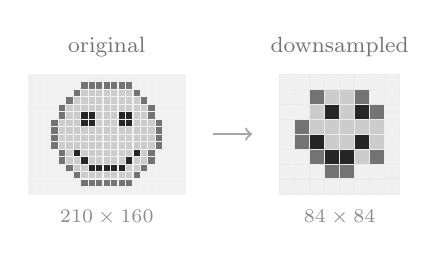
\begin{tikzpicture}[
    lbl/.style={font=\footnotesize, text=black!55},
    dimlbl/.style={font=\scriptsize, text=black!45},
]

% --- Original: 21x16 fine grid (0.095cm cells) ---
\def\cf{0.095}
\foreach \x in {0,...,20} {
    \foreach \y in {0,...,15} {
        \pgfmathsetmacro{\dist}{sqrt((\x-10)*(\x-10)+(\y-7.5)*(\y-7.5))}
        \pgfmathtruncatemacro{\inface}{\dist < 6.3 ? 1 : 0}
        \pgfmathtruncatemacro{\onedge}{(\dist >= 6.3)*(\dist < 7.2) ? 1 : 0}
        \pgfmathtruncatemacro{\feat}{(
            (\x>=7)*(\x<=8)*(\y>=9)*(\y<=10) +
            (\x>=12)*(\x<=13)*(\y>=9)*(\y<=10) +
            (\x==6)*(\y==5) + (\x==14)*(\y==5) +
            (\x==7)*(\y==4) + (\x==13)*(\y==4) +
            (\x>=8)*(\x<=12)*(\y==3)
        ) > 0 ? 1 : 0}
        \ifnum\onedge=1
            \fill[black!55, draw=black!5]
                (\x*\cf, \y*\cf) rectangle ++(\cf, \cf);
        \else\ifnum\inface=0
            \fill[black!6, draw=black!5]
                (\x*\cf, \y*\cf) rectangle ++(\cf, \cf);
        \else\ifnum\feat=1
            \fill[black!85, draw=black!5]
                (\x*\cf, \y*\cf) rectangle ++(\cf, \cf);
        \else
            \fill[black!20, draw=black!5]
                (\x*\cf, \y*\cf) rectangle ++(\cf, \cf);
        \fi\fi\fi
    }
}
\node[lbl] at ({10.5*\cf}, {16*\cf + 0.35}) {original};
\node[dimlbl, anchor=north] at ({10.5*\cf}, -0.08)
    {$210 \times 160$};

% --- Arrow ---
\draw[->, thick, black!35]
    ({21*\cf + 0.35}, {8*\cf}) -- ++(0.5, 0);

% --- Downsampled: 8x8 coarse grid (0.19cm cells, same height) ---
\def\cc{0.19}
\pgfmathsetmacro{\ox}{21*\cf + 1.2}
\pgfmathsetmacro{\oy}{0}
\foreach \x in {0,...,7} {
    \foreach \y in {0,...,7} {
        % Scaled from 21x16: center (3.8, 3.75), radius ~2.4/2.7
        \pgfmathsetmacro{\dist}{sqrt((\x-3.8)*(\x-3.8)+(\y-3.75)*(\y-3.75))}
        \pgfmathtruncatemacro{\inface}{\dist < 2.5 ? 1 : 0}
        \pgfmathtruncatemacro{\onedge}{(\dist >= 2.5)*(\dist < 2.9) ? 1 : 0}
        % Eyes and mouth scaled proportionally from 21x16
        \pgfmathtruncatemacro{\feat}{(
            (\x==3)*(\y==5) + (\x==5)*(\y==5) +
            (\x==2)*(\y==3) + (\x==5)*(\y==3) +
            (\x>=3)*(\x<=4)*(\y==2)
        ) > 0 ? 1 : 0}
        \ifnum\onedge=1
            \fill[black!55, draw=black!8]
                ({\ox + \x*\cc}, {\oy + \y*\cc}) rectangle ++(\cc, \cc);
        \else\ifnum\inface=0
            \fill[black!6, draw=black!8]
                ({\ox + \x*\cc}, {\oy + \y*\cc}) rectangle ++(\cc, \cc);
        \else\ifnum\feat=1
            \fill[black!85, draw=black!8]
                ({\ox + \x*\cc}, {\oy + \y*\cc}) rectangle ++(\cc, \cc);
        \else
            \fill[black!20, draw=black!8]
                ({\ox + \x*\cc}, {\oy + \y*\cc}) rectangle ++(\cc, \cc);
        \fi\fi\fi
    }
}
\node[lbl] at ({\ox + 4*\cc}, {8*\cc + 0.35}) {downsampled};
\node[dimlbl, anchor=north] at ({\ox + 4*\cc}, {\oy - 0.08})
    {$84 \times 84$};

\end{tikzpicture}
\caption{Downsampling. The frame is resized from $210 \times 160$
  to $84 \times 84$. Both images show the same content; the
  downsampled version has fewer, larger pixels.}
\label{fig:resize}
\end{figure}


\smallskip
Fourth, the four most recent preprocessed frames are stacked along
the channel dimension, producing an $84 \times 84 \times 4$ input
tensor. A single frame is a static image -- it shows positions but
not velocities. Stacking four frames gives the network access to
motion information: the direction and speed of a moving object can
be inferred from its positions across consecutive frames, without
requiring recurrence or explicit motion estimation
(\cref{fig:frame-stacking}).
\Cref{fig:preprocessing} summarizes the four steps.

\begin{figure}[ht]
\centering
% Thesis-wide categorical color palette
% Usage: % Thesis-wide categorical color palette
% Usage: \input{figures/palette} in any figure file
%
% Muted primary colors -- print-friendly, visually distinct.
% Inspired by Cooper Union's red/blue primaries, softened for
% academic figures. Use palA-palC for data series in scatter
% plots, line charts, bar charts, etc.

\definecolor{palA}{HTML}{1F77B4}   % Tableau blue
\definecolor{palB}{HTML}{D62728}   % Tableau red
\definecolor{palC}{HTML}{2CA02C}   % Tableau green
 in any figure file
%
% Muted primary colors -- print-friendly, visually distinct.
% Inspired by Cooper Union's red/blue primaries, softened for
% academic figures. Use palA-palC for data series in scatter
% plots, line charts, bar charts, etc.

\definecolor{palA}{HTML}{1F77B4}   % Tableau blue
\definecolor{palB}{HTML}{D62728}   % Tableau red
\definecolor{palC}{HTML}{2CA02C}   % Tableau green


%% Panel (a): Filmstrip of 4 frames with ball at different positions
\begin{subfigure}{\textwidth}
\centering
\begin{tikzpicture}[
    lbl/.style={font=\footnotesize, text=black!55},
    dimlbl/.style={font=\scriptsize, text=black!45},
    tlbl/.style={font=\scriptsize, text=black!50},
]
\def\c{0.28}
\def\gs{5}  % 5x5 grid per frame

% Draw one frame: #1=x-offset, #2=ball-x (grid coords), #3=ball-y, #4=opacity
\newcommand{\drawframe}[4]{
    \foreach \x in {0,...,4} {
        \foreach \y in {0,...,4} {
            \fill[black!5, draw=black!12]
                ({#1 + \x*\c}, \y*\c) rectangle ++(\c, \c);
        }
    }
    % Ball
    \fill[palA!#4] ({#1 + (#2+0.5)*\c}, {(#3+0.5)*\c}) circle (0.11);
}

% Four frames with ball moving diagonally
\drawframe{0}{1}{1}{30}        % t-3: bottom-left
\drawframe{1.7}{2}{2}{45}      % t-2: center-left
\drawframe{3.4}{3}{3}{60}      % t-1: center-right
\drawframe{5.1}{4}{4}{100}     % t:   top-right

% Time labels below each frame
\node[tlbl] at ({2.5*\c}, {-0.2}) {$t{-}3$};
\node[tlbl] at ({1.7 + 2.5*\c}, {-0.2}) {$t{-}2$};
\node[tlbl] at ({3.4 + 2.5*\c}, {-0.2}) {$t{-}1$};
\node[tlbl] at ({5.1 + 2.5*\c}, {-0.2}) {$t$};

% Arrow to stacked output
\draw[->, thick, black!40]
    ({5.1 + 5*\c + 0.25}, {2.5*\c}) -- ++(0.5, 0);

% Output block
\node[draw=black!30, thick, rounded corners=2pt,
      minimum width=1.1cm, minimum height=1.3cm,
      fill=black!5, font=\scriptsize, align=center]
    at ({5.1 + 5*\c + 1.35}, {2.5*\c})
    {$84{\times}84$\\${\times}\,4$};

\end{tikzpicture}
\subcaption{Four consecutive frames capture the ball at different
  positions. Stacking them produces one multi-channel input.}
\label{fig:frame-stack-op}
\end{subfigure}

\vspace{1em}

%% Panel (b): Motion inference from the stacked frames
\begin{subfigure}{\textwidth}
\centering
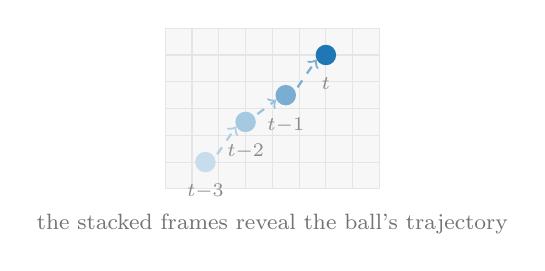
\begin{tikzpicture}[
    lbl/.style={font=\footnotesize, text=black!55},
    dimlbl/.style={font=\scriptsize, text=black!45},
]
\def\c{0.34}

% Game-like grid (8x6)
\foreach \x in {0,...,7} {
    \foreach \y in {0,...,5} {
        \fill[gray!6, draw=black!10]
            (\x*\c, \y*\c) rectangle ++(\c, \c);
    }
}

% Ball at four positions matching panel (a), increasing opacity
% t-3: bottom-left
\fill[palA!25] ({1.5*\c}, {1*\c}) circle (0.13);
\node[dimlbl, anchor=north] at ({1.5*\c}, {1*\c - 0.16})
    {$t{-}3$};

% t-2: left-center
\fill[palA!40] ({3*\c}, {2.5*\c}) circle (0.13);
\node[dimlbl, anchor=north] at ({3*\c}, {2.5*\c - 0.16})
    {$t{-}2$};

% t-1: right-center
\fill[palA!60] ({4.5*\c}, {3.5*\c}) circle (0.13);
\node[dimlbl, anchor=north] at ({4.5*\c}, {3.5*\c - 0.16})
    {$t{-}1$};

% t: upper-right
\fill[palA] ({6*\c}, {5*\c}) circle (0.13);
\node[dimlbl, anchor=north] at ({6*\c}, {5*\c - 0.16})
    {$t$};

% Dashed trajectory arrows
\draw[->, thick, dashed, palA!35]
    ({1.5*\c + 0.15}, {1*\c + 0.1})
    -- ({3*\c - 0.12}, {2.5*\c - 0.06});
\draw[->, thick, dashed, palA!45]
    ({3*\c + 0.15}, {2.5*\c + 0.1})
    -- ({4.5*\c - 0.12}, {3.5*\c - 0.06});
\draw[->, thick, dashed, palA!60]
    ({4.5*\c + 0.15}, {3.5*\c + 0.1})
    -- ({6*\c - 0.12}, {5*\c - 0.06});

% Annotation
\node[lbl, anchor=north, align=center] at ({4*\c}, -0.2)
    {the stacked frames reveal the ball's trajectory};

\end{tikzpicture}
\subcaption{Overlaying the four frames shows the ball's direction
  -- information unavailable from any single frame.}
\label{fig:frame-stack-motion}
\end{subfigure}

\caption{Frame stacking provides motion information.
  (a)~Each frame captures a snapshot; stacking concatenates them.
  (b)~The network reads velocity from positions across frames.}
\label{fig:frame-stacking}
\end{figure}


\begin{figure}[ht]
\centering
% Thesis-wide categorical color palette
% Usage: % Thesis-wide categorical color palette
% Usage: \input{figures/palette} in any figure file
%
% Muted primary colors -- print-friendly, visually distinct.
% Inspired by Cooper Union's red/blue primaries, softened for
% academic figures. Use palA-palC for data series in scatter
% plots, line charts, bar charts, etc.

\definecolor{palA}{HTML}{1F77B4}   % Tableau blue
\definecolor{palB}{HTML}{D62728}   % Tableau red
\definecolor{palC}{HTML}{2CA02C}   % Tableau green
 in any figure file
%
% Muted primary colors -- print-friendly, visually distinct.
% Inspired by Cooper Union's red/blue primaries, softened for
% academic figures. Use palA-palC for data series in scatter
% plots, line charts, bar charts, etc.

\definecolor{palA}{HTML}{1F77B4}   % Tableau blue
\definecolor{palB}{HTML}{D62728}   % Tableau red
\definecolor{palC}{HTML}{2CA02C}   % Tableau green

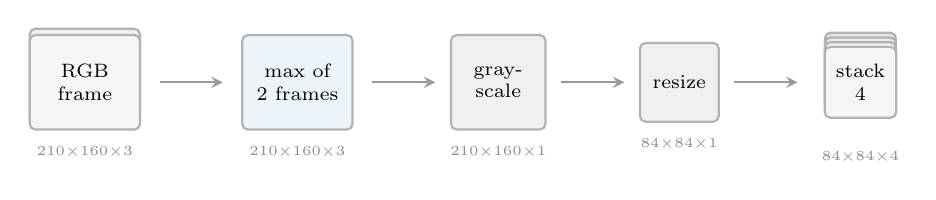
\begin{tikzpicture}[
    box/.style={draw=black!30, thick, minimum height=1.2cm,
                font=\scriptsize, inner sep=4pt, align=center,
                rounded corners=2pt},
    arr/.style={->, thick, >=stealth, black!40},
    dimlbl/.style={font=\tiny, text=black!45},
]

% Raw frames (two overlapping)
\node[box, minimum width=1.4cm, fill=black!6]
    (raw2) at (0, 0.08) {};
\node[box, minimum width=1.4cm, fill=black!4]
    (raw1) at (0, 0) {RGB\\frame};
\node[dimlbl, below=2pt] at (raw1.south)
    {210${\times}$160${\times}$3};

\draw[arr] (0.95, 0) -- (1.75, 0);

% Max of two frames
\node[box, minimum width=1.4cm, fill=palA!8]
    (maxf) at (2.7, 0) {max of\\2 frames};
\node[dimlbl, below=2pt] at (maxf.south)
    {210${\times}$160${\times}$3};

\draw[arr] (3.65, 0) -- (4.45, 0);

% Grayscale
\node[box, minimum width=1.2cm, fill=black!6]
    (gray) at (5.25, 0) {gray-\\scale};
\node[dimlbl, below=2pt] at (gray.south)
    {210${\times}$160${\times}$1};

\draw[arr] (6.05, 0) -- (6.85, 0);

% Resize
\node[box, minimum width=1.0cm, minimum height=1.0cm,
      fill=black!6]
    (resize) at (7.55, 0) {resize};
\node[dimlbl, below=2pt] at (resize.south)
    {84${\times}$84${\times}$1};

\draw[arr] (8.25, 0) -- (9.05, 0);

% Stack 4 frames (four overlapping boxes)
\node[box, minimum width=0.9cm, minimum height=0.9cm,
      fill=black!10] at (9.85, 0.18) {};
\node[box, minimum width=0.9cm, minimum height=0.9cm,
      fill=black!8] at (9.85, 0.12) {};
\node[box, minimum width=0.9cm, minimum height=0.9cm,
      fill=black!6] at (9.85, 0.06) {};
\node[box, minimum width=0.9cm, minimum height=0.9cm,
      fill=black!4]
    (stack) at (9.85, 0) {stack\\4};
\node[dimlbl, below=8pt] at (stack.south)
    {84${\times}$84${\times}$4};

\end{tikzpicture}
\caption{Preprocessing pipeline. Two consecutive raw frames are
  combined, converted to grayscale, resized, and stacked to produce
  the input tensor for the network.}
\label{fig:preprocessing}
\end{figure}


\smallskip
This preprocessing pipeline has become standard in deep reinforcement
learning for visual environments -- virtually every subsequent
method, including those discussed in later sections, uses the same
four steps~\citep{mnih2015human}.

\subsection{The DQN Architecture}
\label{subsec:dqn-architecture}

The preprocessed $84 \times 84 \times 4$ tensor is the input to
the \emph{Nature CNN}, a convolutional neural network introduced
by~\citet{mnih2015human}. The architecture uses the convolutional
layers described in \cref{subsec:conv-layers}: three convolutional
layers that extract spatial features while progressively reducing
the spatial dimensions, followed by a fully connected layer and a
linear output layer. The three convolutional layers use 32, 64,
and 64 filters with kernel sizes of $8 \times 8$, $4 \times 4$,
and $3 \times 3$ and strides of 4, 2, and 1, respectively. The
large kernel and stride in the first layer rapidly reduce the
spatial dimensions from $84 \times 84$ to $20 \times 20$, producing
$32$ feature maps; the later layers refine features at finer spatial
scales.

\smallskip After the final convolutional
layer, the output is flattened and passed through a fully connected
layer with 512 units. Each hidden layer uses a ReLU activation
function. The output layer produces one Q-value for every available
action -- typically 18 for standard game environments.
\Cref{fig:nature-cnn} shows the architecture visually, and
\cref{tab:nature-cnn-layers} lists the exact specifications.

\begin{figure}[ht]
\centering
\definecolor{convfront}{HTML}{B8CCE4}
\definecolor{convtop}{HTML}{D0DEF0}
\definecolor{convside}{HTML}{8FAEC8}
\definecolor{fcfront}{HTML}{C5D5C5}
\definecolor{fctop}{HTML}{D8E6D8}
\definecolor{fcside}{HTML}{9AB89A}
\definecolor{outfront}{HTML}{D4C5B0}
\definecolor{outtop}{HTML}{E4D8C8}
\definecolor{outside}{HTML}{B8A890}
\resizebox{0.85\textwidth}{!}{%
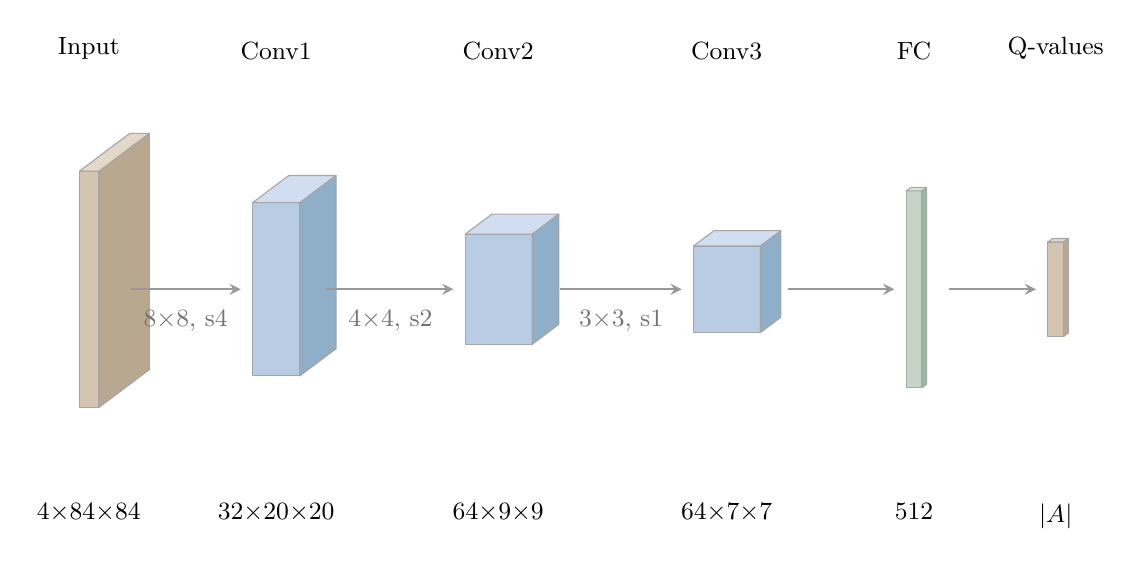
\begin{tikzpicture}[
    x={(1cm,0cm)}, y={(0cm,1cm)}, z={(0.4cm,0.3cm)},
    arr/.style={->, thick, >=stealth, black!40},
    dimlbl/.style={font=\small, anchor=north},
    namelbl/.style={font=\small, anchor=south},
    filtlbl/.style={font=\small, text=black!55, anchor=north}
]

\newcommand{\cuboid}[7]{
    \fill[#5, draw=black!35, line join=round]
        (#1, {-#3/2}, 0) -- ({#1+#2}, {-#3/2}, 0) --
        ({#1+#2}, {#3/2}, 0) -- (#1, {#3/2}, 0) -- cycle;
    \fill[#6, draw=black!35, line join=round]
        (#1, {#3/2}, 0) -- ({#1+#2}, {#3/2}, 0) --
        ({#1+#2}, {#3/2}, #4) -- (#1, {#3/2}, #4) -- cycle;
    \fill[#7, draw=black!35, line join=round]
        ({#1+#2}, {-#3/2}, 0) -- ({#1+#2}, {#3/2}, 0) --
        ({#1+#2}, {#3/2}, #4) -- ({#1+#2}, {-#3/2}, #4) -- cycle;
}

% Baselines
\def\dimY{-2.6}
\def\nameY{2.8}

% Input: 4 x 84 x 84
\cuboid{0.8}{0.25}{3.0}{1.6}{outfront}{outtop}{outside}
\node[namelbl] at (0.92, \nameY, 0) {Input};
\node[dimlbl] at (0.92, \dimY, 0) {4${\times}$84${\times}$84};

% Arrow + label below
\draw[arr] (1.45, 0, 0) -- (2.85, 0, 0);
\node[filtlbl] at (2.15, -0.15, 0) {8${\times}$8, s4};

% Conv1: 32 x 20 x 20
\cuboid{3.0}{0.6}{2.2}{1.15}{convfront}{convtop}{convside}
\node[namelbl] at (3.3, \nameY, 0) {Conv1};
\node[dimlbl] at (3.3, \dimY, 0) {32${\times}$20${\times}$20};

% Arrow + label below
\draw[arr] (3.95, 0, 0) -- (5.55, 0, 0);
\node[filtlbl] at (4.75, -0.15, 0) {4${\times}$4, s2};

% Conv2: 64 x 9 x 9
\cuboid{5.7}{0.85}{1.4}{0.85}{convfront}{convtop}{convside}
\node[namelbl] at (6.12, \nameY, 0) {Conv2};
\node[dimlbl] at (6.12, \dimY, 0) {64${\times}$9${\times}$9};

% Arrow + label below
\draw[arr] (6.9, 0, 0) -- (8.45, 0, 0);
\node[filtlbl] at (7.68, -0.15, 0) {3${\times}$3, s1};

% Conv3: 64 x 7 x 7
\cuboid{8.6}{0.85}{1.1}{0.65}{convfront}{convtop}{convside}
\node[namelbl] at (9.02, \nameY, 0) {Conv3};
\node[dimlbl] at (9.02, \dimY, 0) {64${\times}$7${\times}$7};

% Arrow
\draw[arr] (9.8, 0, 0) -- (11.15, 0, 0);

% FC: 512
\cuboid{11.3}{0.2}{2.5}{0.15}{fcfront}{fctop}{fcside}
\node[namelbl] at (11.4, \nameY, 0) {FC};
\node[dimlbl] at (11.4, \dimY, 0) {512};

% Arrow
\draw[arr] (11.85, 0, 0) -- (12.95, 0, 0);

% Q-values
\cuboid{13.1}{0.2}{1.2}{0.15}{outfront}{outtop}{outside}
\node[namelbl] at (13.2, \nameY, 0) {Q-values};
\node[dimlbl] at (13.2, \dimY, 0) {$|A|$};

\end{tikzpicture}%
}
\caption{Nature CNN architecture. Block height reflects spatial
  dimensions; block depth reflects channel count. All convolutional
  and fully connected layers use ReLU activation.}
\label{fig:nature-cnn}
\end{figure}

\begin{table}[ht]
\centering
\renewcommand{\arraystretch}{1.4}
\begin{tabular}{llcccc}
\toprule
Layer & Type & Filters & Kernel & Stride & Output \\
\midrule
Input    & --             & --  & --            & --  & $4 \times 84 \times 84$ \\
Conv1    & Conv2d + ReLU  & 32  & $8 \times 8$  & 4   & $32 \times 20 \times 20$ \\
Conv2    & Conv2d + ReLU  & 64  & $4 \times 4$  & 2   & $64 \times 9 \times 9$ \\
Conv3    & Conv2d + ReLU  & 64  & $3 \times 3$  & 1   & $64 \times 7 \times 7$ \\
Flatten  & --             & --  & --            & --  & 3136 \\
FC       & Linear + ReLU  & --  & --            & --  & 512 \\
Q-head   & Linear         & --  & --            & --  & $|A|$ \\
\bottomrule
\end{tabular}
\caption{Nature CNN layer specifications. Each convolutional layer
  applies the listed kernel with the given stride, followed by ReLU
  activation. The output layer is linear.}
\label{tab:nature-cnn-layers}
\end{table}


\smallskip
This all-actions output design is a deliberate architectural choice.
Rather than taking a state--action pair as input and outputting a
single Q-value, the network takes only the state and produces all
Q-values in one forward pass. Computing
$\max_a Q(s, a;\, \mathbf{w})$ -- needed for both the greedy policy
and the TD target -- therefore requires a single pass through the
network, not $|\mathcal{A}|$ separate passes.

\smallskip
The convolutional layers serve as the encoder described in
\cref{subsec:representations}: a learned feature extractor that
compresses the game frame into a 512-dimensional representation.
This representation captures whatever spatial structure is relevant
for predicting Q-values, and it is shaped entirely by the TD error
from \cref{eq:fa-loss} -- the Q-learning loss is the only training
signal that drives the encoder. Whether this signal alone
produces representations that capture the full structure of the
environment, or whether additional self-supervised objectives can
improve them, is a central question in data-efficient reinforcement
learning.

\subsection{Experience Replay}
\label{subsec:experience-replay-bg}

The previous section described the architecture that maps raw frames
to Q-values. But training this network with standard Q-learning
updates -- applying the SGD rule from \cref{eq:sgd-update} to each
transition as it arrives -- is unstable. The problem lies not in the
network itself, but in the data it trains on.

\smallskip
In supervised learning, SGD convergence relies on the training data
being independent and identically distributed (i.i.d.): each example
in a minibatch is drawn independently from the same underlying
distribution. In reinforcement learning, this assumption is violated
in two ways.

\smallskip
First, consecutive transitions are highly correlated. If the agent
is in a particular state at time~$t$, the state at time~$t+1$ is
almost identical -- a ball has moved a few pixels, or a character has
shifted slightly. Training on a sequence of near-identical inputs
pushes the network's parameters in the same direction repeatedly,
overfitting to the agent's recent local experience rather than
learning general value estimates.

\smallskip
Second, the data distribution itself changes as the agent learns.
Each gradient step updates the network, which changes the policy,
which changes which states the agent visits, which changes the
distribution of training data. The agent is training on a shifting
distribution of its own creation -- a feedback loop that can cause
the network's predictions to diverge.

\smallskip
\emph{Experience replay}~\citep{lin1992self,mnih2013playing} breaks
this loop with a simple mechanism: instead of training on each
transition once as it arrives, the agent stores every transition
$(s, a, r, s')$ in a large buffer and trains on random minibatches
sampled uniformly from the buffer. The buffer is a fixed-size
first-in-first-out queue -- typically holding one million transitions.
When full, the oldest transitions are discarded to make room for
new ones. \Cref{fig:replay-buffer} illustrates the mechanism:
transitions arrive sequentially from the agent, but the training
minibatch is assembled by sampling randomly across the buffer.

\begin{figure}[ht]
\centering
% Thesis-wide categorical color palette
% Usage: % Thesis-wide categorical color palette
% Usage: \input{figures/palette} in any figure file
%
% Muted primary colors -- print-friendly, visually distinct.
% Inspired by Cooper Union's red/blue primaries, softened for
% academic figures. Use palA-palC for data series in scatter
% plots, line charts, bar charts, etc.

\definecolor{palA}{HTML}{1F77B4}   % Tableau blue
\definecolor{palB}{HTML}{D62728}   % Tableau red
\definecolor{palC}{HTML}{2CA02C}   % Tableau green
 in any figure file
%
% Muted primary colors -- print-friendly, visually distinct.
% Inspired by Cooper Union's red/blue primaries, softened for
% academic figures. Use palA-palC for data series in scatter
% plots, line charts, bar charts, etc.

\definecolor{palA}{HTML}{1F77B4}   % Tableau blue
\definecolor{palB}{HTML}{D62728}   % Tableau red
\definecolor{palC}{HTML}{2CA02C}   % Tableau green

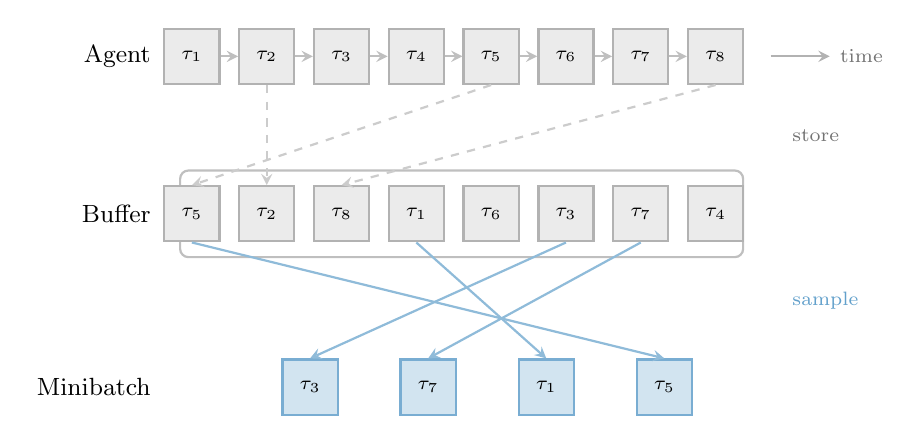
\begin{tikzpicture}[
    trans/.style={draw=black!30, thick, minimum width=0.7cm,
                  minimum height=0.7cm, font=\scriptsize,
                  inner sep=0pt, fill=black!8},
    arr/.style={->, thick, >=stealth},
    lbl/.style={font=\small},
    sublbl/.style={font=\scriptsize, text=black!55},
]

% --- Timeline (top) ---
\node[lbl, anchor=east] at (-0.4, 0) {Agent};
\node[trans] (t1) at (0, 0)    {$\tau_{1}$};
\node[trans] (t2) at (0.95, 0) {$\tau_{2}$};
\node[trans] (t3) at (1.90, 0) {$\tau_{3}$};
\node[trans] (t4) at (2.85, 0) {$\tau_{4}$};
\node[trans] (t5) at (3.80, 0) {$\tau_{5}$};
\node[trans] (t6) at (4.75, 0) {$\tau_{6}$};
\node[trans] (t7) at (5.70, 0) {$\tau_{7}$};
\node[trans] (t8) at (6.65, 0) {$\tau_{8}$};

\foreach \i in {1,...,7} {
    \pgfmathtruncatemacro{\next}{\i+1}
    \draw[arr, black!25] (t\i.east) -- (t\next.west);
}

% "time" arrow
\draw[arr, black!30] (7.35, 0) -- (8.1, 0)
    node[right, sublbl] {time};

% --- Buffer (middle) ---
\node[lbl, anchor=east] at (-0.4, -2) {Buffer};

% Buffer outline
\draw[thick, black!25, rounded corners=3pt]
    (-0.15, -2.55) rectangle (7.0, -1.45);

% Transitions in buffer (shuffled order)
\node[trans] (b5) at (0, -2)    {$\tau_{5}$};
\node[trans] (b2) at (0.95, -2) {$\tau_{2}$};
\node[trans] (b8) at (1.90, -2) {$\tau_{8}$};
\node[trans] (b1) at (2.85, -2) {$\tau_{1}$};
\node[trans] (b6) at (3.80, -2) {$\tau_{6}$};
\node[trans] (b3) at (4.75, -2) {$\tau_{3}$};
\node[trans] (b7) at (5.70, -2) {$\tau_{7}$};
\node[trans] (b4) at (6.65, -2) {$\tau_{4}$};

% Store arrows (a few representative ones)
\draw[arr, black!20, dashed] (t2.south) -- (b2.north);
\draw[arr, black!20, dashed] (t5.south) -- (b5.north);
\draw[arr, black!20, dashed] (t8.south) -- (b8.north);
\node[sublbl, right] at (7.5, -1.0) {store};

% --- Minibatch (bottom) ---
\node[lbl, anchor=east] at (-0.4, -4.2) {Minibatch};

% Sampled transitions (non-consecutive)
\node[trans, fill=palA!20, draw=palA!60]
    (m1) at (1.5, -4.2) {$\tau_{3}$};
\node[trans, fill=palA!20, draw=palA!60]
    (m2) at (3.0, -4.2) {$\tau_{7}$};
\node[trans, fill=palA!20, draw=palA!60]
    (m3) at (4.5, -4.2) {$\tau_{1}$};
\node[trans, fill=palA!20, draw=palA!60]
    (m4) at (6.0, -4.2) {$\tau_{5}$};

% Sample arrows
\draw[arr, palA!50] (b3.south) -- (m1.north);
\draw[arr, palA!50] (b7.south) -- (m2.north);
\draw[arr, palA!50] (b1.south) -- (m3.north);
\draw[arr, palA!50] (b5.south) -- (m4.north);
\node[sublbl, right, text=palA!70] at (7.5, -3.1) {sample};

\end{tikzpicture}
\caption{Experience replay. Transitions arrive sequentially and are
  stored in a buffer. Training minibatches are sampled randomly,
  breaking the temporal correlations.}
\label{fig:replay-buffer}
\end{figure}


\smallskip
Random sampling from the buffer serves three purposes. First, it
\emph{decorrelates} the training data: a minibatch drawn from a
million-transition buffer contains experiences from many different
episodes and time steps, approximating the i.i.d.\ condition that
SGD requires.

\smallskip
Second, it improves \emph{data efficiency}: each transition can
appear in many minibatches over the course of training, rather than
being used for a single gradient step and discarded. This is
especially important when environment interactions are expensive --
extracting more learning from each transition means the agent needs
fewer total interactions to improve.

\smallskip
Third, it provides \emph{smoothing}: because the buffer accumulates
transitions from many past versions of the policy, the training
distribution changes gradually rather than shifting abruptly with
each policy update. This prevents the network from overfitting to
its most recent behavior and reduces oscillations in the learned
values.

\smallskip
Experience replay connects directly to the function approximation
loss in \cref{eq:fa-loss}. That equation defined the expected
squared TD error, with the expectation taken over transitions --
but did not specify where those transitions come from. Experience
replay provides the answer: the expectation is approximated by
sampling minibatches from the buffer, and each sampled transition
contributes one term to the loss.

\subsection{Data Augmentation}
\label{subsec:data-augmentation}

When training data is limited, the agent replays the same transitions
repeatedly, risking overfitting to specific pixel patterns rather than
learning general features. Data augmentation -- applying small,
semantics-preserving transformations to game frames during training --
expands the effective dataset without additional environment interaction.

\smallskip
In supervised learning, data augmentation applies label-preserving
transformations to training inputs: random crops, horizontal flips,
color jitter. The key requirement is that the transformation must
not change the correct answer -- a horizontally flipped cat is
still a cat. Augmentation is standard practice for training image
classifiers, especially when data is limited, because it
effectively multiplies the dataset by creating many versions of
each training example.

\smallskip
Transferring this idea to reinforcement learning is not
straightforward. In supervised learning, the label for an image is
fixed: a cat is always a cat regardless of how many times the image
is transformed. In RL, the ``label'' for an observation is the
Q-value target, which depends on the current policy and changes
every training step. But the observation itself is still an image.
If a small spatial transformation does not change the game
semantics -- the paddle is in nearly the same position, the ball
trajectory is the same, the optimal action has not changed -- then
the Q-values should also be unchanged. Spatial transforms that
produce small, semantics-preserving perturbations should therefore
be safe for RL, despite the non-stationary target problem.

\smallskip
The specific augmentation used in data-efficient RL is the
\emph{random shift}. Starting from the preprocessed
$84 \times 84$ grayscale frame, the operation pads the image by 4
pixels on each side using reflection padding, creating a
$92 \times 92$ image where the border mirrors the edge pixels.
Reflection is used rather than zero padding because it fills the
border with plausible image content -- mirrored textures and edges
-- rather than artificial black pixels that the encoder could learn
to detect as a padding signal rather than game content. A
random $84 \times 84$ crop is then taken from this padded image,
with the crop position sampled uniformly at random. The result is
the original game frame shifted by up to $\pm 4$ pixels in both the
horizontal and vertical directions. The visual content is preserved;
only the spatial position has changed slightly.
\Cref{fig:random-shift} illustrates the three steps. This is the
operation used by DrQ~\citep{kostrikov2020image}; the equivalent
operation in RAD~\citep{laskin2020reinforcement} is called ``random
translate.''

\begin{figure}[htbp]
\centering
% Thesis-wide categorical color palette
% Usage: % Thesis-wide categorical color palette
% Usage: \input{figures/palette} in any figure file
%
% Muted primary colors -- print-friendly, visually distinct.
% Inspired by Cooper Union's red/blue primaries, softened for
% academic figures. Use palA-palC for data series in scatter
% plots, line charts, bar charts, etc.

\definecolor{palA}{HTML}{1F77B4}   % Tableau blue
\definecolor{palB}{HTML}{D62728}   % Tableau red
\definecolor{palC}{HTML}{2CA02C}   % Tableau green
 in any figure file
%
% Muted primary colors -- print-friendly, visually distinct.
% Inspired by Cooper Union's red/blue primaries, softened for
% academic figures. Use palA-palC for data series in scatter
% plots, line charts, bar charts, etc.

\definecolor{palA}{HTML}{1F77B4}   % Tableau blue
\definecolor{palB}{HTML}{D62728}   % Tableau red
\definecolor{palC}{HTML}{2CA02C}   % Tableau green


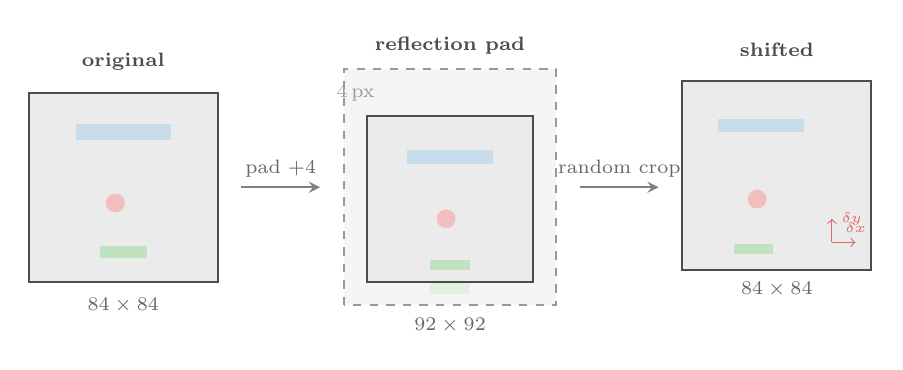
\begin{tikzpicture}[
    arr/.style={->, thick, >=stealth, black!50},
    lbl/.style={font=\scriptsize, text=black!60},
]

% === Panel 1: Original 84x84 ===
\draw[thick, black!70, fill=black!8]
    (0, 0) rectangle (2.4, 2.4);
% Content region schematic (simple game elements)
\fill[palA!25] (0.6, 1.8) rectangle (1.8, 2.0);  % top bar
\fill[palB!30] (1.1, 1.0) circle (0.12);          % ball
\fill[palC!30] (0.9, 0.3) rectangle (1.5, 0.45);  % paddle
\node[lbl] at (1.2, -0.3) {$84 \times 84$};
\node[font=\scriptsize\bfseries, text=black!70] at (1.2, 2.8)
    {original};

% Arrow 1
\draw[arr] (2.7, 1.2) -- node[above, lbl] {pad $+4$} (3.7, 1.2);

% === Panel 2: Padded 92x92 ===
% Padding region (lighter)
\draw[thick, black!40, fill=black!4, dashed]
    (4.0, -0.3) rectangle (6.7, 2.7);
% Original content region inside padding
\draw[thick, black!70, fill=black!8]
    (4.3, 0.0) rectangle (6.4, 2.1);
% Same game elements (shifted inward)
\fill[palA!25] (4.8, 1.5) rectangle (5.9, 1.67);
\fill[palB!30] (5.3, 0.8) circle (0.12);
\fill[palC!30] (5.1, 0.15) rectangle (5.6, 0.28);
% Reflection hint (mirrored paddle at bottom edge)
\fill[palC!15] (5.1, -0.15) rectangle (5.6, -0.02);
% Dimension labels
\node[lbl] at (5.35, -0.55) {$92 \times 92$};
% Padding annotation
\node[lbl, text=black!40] at (4.15, 2.4) {4\,px};
\node[font=\scriptsize\bfseries, text=black!70] at (5.35, 3.0)
    {reflection pad};

% Arrow 2
\draw[arr] (7.0, 1.2) -- node[above, lbl] {random crop} (8.0, 1.2);

% === Panel 3: Cropped 84x84 (shifted) ===
% Show a slightly offset crop
\draw[thick, black!70, fill=black!8]
    (8.3, 0.15) rectangle (10.7, 2.55);
% Same elements but shifted by ~2px equivalent
\fill[palA!25] (8.75, 1.9) rectangle (9.85, 2.07);
\fill[palB!30] (9.25, 1.05) circle (0.12);
\fill[palC!30] (8.95, 0.35) rectangle (9.45, 0.48);
\node[lbl] at (9.5, -0.1) {$84 \times 84$};
\node[font=\scriptsize\bfseries, text=black!70] at (9.5, 2.95)
    {shifted};

% Offset annotation (small arrows showing dx, dy)
\draw[->, thin, palB!70] (10.2, 0.5) -- (10.2, 0.8)
    node[right, font=\tiny, text=palB!70] {$\delta y$};
\draw[->, thin, palB!70] (10.2, 0.5) -- (10.5, 0.5)
    node[above, font=\tiny, text=palB!70] {$\delta x$};

\end{tikzpicture}
\caption{Random shift augmentation. The $84 \times 84$ frame is
  padded by 4 pixels on each side using reflection, then randomly
  cropped back to $84 \times 84$, producing a small spatial shift.}
\label{fig:random-shift}
\end{figure}


\smallskip
Because the observation is a stack of four consecutive frames, the
same random shift -- the same horizontal and vertical offset -- is
applied to all four frames in the stack. This consistency matters:
the agent infers velocity and motion from pixel differences between
consecutive frames. If each frame were shifted independently, these
inter-frame differences would be corrupted, creating spurious
motion signals. Consistent augmentation across the stack preserves
temporal information while still providing spatial perturbation.

\smallskip
During training, each transition $(s, a, r, s')$ sampled from the
replay buffer is augmented before computing the loss. The current
state $s$ and next state $s'$ receive independent random shifts --
different crop positions -- because they are separate observations.
There is no need for the spatial offset of $s$ and $s'$ to match.
Both DrQ and RAD apply augmentation in this way.

\smallskip
\citet{laskin2020reinforcement} systematically tested ten
augmentation types on pixel-based RL: crop, translate, window,
grayscale, cutout, cutout-color, flip, rotate, random convolution,
and color jitter. Random crop and translate were the most effective
by a wide margin; most other augmentations were neutral or harmful.
The reason is that game semantics are approximately
translation-invariant at small scales -- a paddle shifted three
pixels is still a paddle in approximately the same place -- but
they are not invariant to other transforms. Horizontal flips
reverse left and right, changing the optimal action. Rotation
disrupts spatial layout (gravity goes sideways). Color jitter
alters object appearance in ways the encoder should remain
sensitive to. Random shift succeeds because it perturbs position
without breaking the game's spatial structure.

\smallskip
DrQ~\citep{kostrikov2020image} and
RAD~\citep{laskin2020reinforcement} are concurrent papers that
independently demonstrated image augmentation is sufficient for
competitive data-efficient RL. DrQ additionally proposed averaging
Q-targets across $K$ augmented versions of $s'$ and averaging
Q-values across $M$ augmented versions of $s$, but the simplest
setting -- $K = 1$, $M = 1$, a single random shift per observation
-- is already sufficient for Atari-100K. No complex averaging or
multiple forward passes are needed.

\smallskip
In the 100K regime, the replay buffer contains at most around
100{,}000 transitions -- this is the agent's entire dataset. With a
replay ratio of one (one gradient update per environment step),
each transition is sampled roughly once. Data-efficient settings
often use higher replay ratios, reusing each transition two to four
times. When the same transitions are replayed repeatedly, the
network risks memorizing specific pixel patterns rather than
learning general features. This is the same overfitting problem
that afflicts small-dataset classifiers in supervised learning, but
amplified by the shifting target distribution in RL.

\smallskip
Consider what overfitting looks like at the representation level.
The encoder might learn that a bright pixel at position $(42, 17)$
predicts high Q-values -- because in the limited training data,
that pixel happens to be bright when the ball is near the paddle.
This feature is fragile: it breaks with any positional variation.
A robust encoder would instead learn to represent the ball's
position relative to the paddle, a feature that generalizes across
spatial shifts. Without augmentation, the encoder has no pressure
to prefer the robust feature over the fragile one, because both
predict Q-values equally well on the exact training observations.
\Cref{fig:fragile-vs-robust} illustrates this contrast.

\begin{figure}[ht]
\centering
% Thesis-wide categorical color palette
% Usage: % Thesis-wide categorical color palette
% Usage: \input{figures/palette} in any figure file
%
% Muted primary colors -- print-friendly, visually distinct.
% Inspired by Cooper Union's red/blue primaries, softened for
% academic figures. Use palA-palC for data series in scatter
% plots, line charts, bar charts, etc.

\definecolor{palA}{HTML}{1F77B4}   % Tableau blue
\definecolor{palB}{HTML}{D62728}   % Tableau red
\definecolor{palC}{HTML}{2CA02C}   % Tableau green
 in any figure file
%
% Muted primary colors -- print-friendly, visually distinct.
% Inspired by Cooper Union's red/blue primaries, softened for
% academic figures. Use palA-palC for data series in scatter
% plots, line charts, bar charts, etc.

\definecolor{palA}{HTML}{1F77B4}   % Tableau blue
\definecolor{palB}{HTML}{D62728}   % Tableau red
\definecolor{palC}{HTML}{2CA02C}   % Tableau green


%% (a) Fragile: fixed pixel position
\begin{subfigure}[t]{0.47\textwidth}
\centering
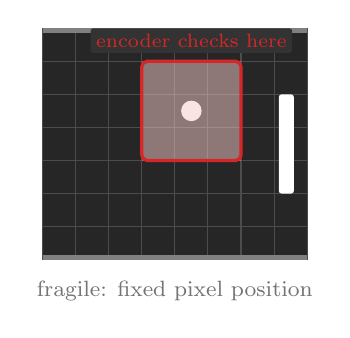
\begin{tikzpicture}[
    lbl/.style={font=\footnotesize, text=black!55},
]
\def\c{0.42}
\def\gw{8}
\def\gh{7}

% Dark game background
\fill[black!85] (0, 0) rectangle ({\gw*\c}, {\gh*\c});
% Subtle grid lines
\foreach \x in {0,...,8} {
    \draw[black!70] (\x*\c, 0) -- (\x*\c, {\gh*\c});
}
\foreach \y in {0,...,7} {
    \draw[black!70] (0, \y*\c) -- ({\gw*\c}, \y*\c);
}

% Top and bottom walls (Pong borders)
\fill[black!50] (0, 0) rectangle ({\gw*\c}, {0.15*\c});
\fill[black!50] (0, {6.85*\c}) rectangle ({\gw*\c}, {\gh*\c});

% Paddle (tall, thin, right side)
\fill[white!90, rounded corners=1pt]
    ({7*\c + 0.06}, {2*\c}) rectangle ({7.6*\c}, {5*\c});

% Ball
\fill[white] ({4.5*\c}, {4.5*\c}) circle (0.13);

% Spotlight: bright region at fixed position (cells 3-5, 3-5)
\fill[palB!25, opacity=0.5]
    ({3*\c}, {3*\c}) rectangle ({6*\c}, {6*\c});
\draw[palB, very thick, rounded corners=2pt]
    ({3*\c}, {3*\c}) rectangle ({6*\c}, {6*\c});

% Label on spotlight
\node[font=\scriptsize, text=palB, fill=black!80,
      inner sep=2pt, rounded corners=1pt, anchor=south]
    at ({4.5*\c}, {6*\c + 0.1})
    {encoder checks here};

% Verdict
\node[lbl] at ({4*\c}, {-0.4})
    {fragile: fixed pixel position};

\end{tikzpicture}
\subcaption{The encoder memorizes a fixed region. It works when
  the ball is there but fails if the image shifts.}
\label{fig:fragile-feature}
\end{subfigure}
\hfill
%% (b) Robust: object relationship
\begin{subfigure}[t]{0.47\textwidth}
\centering
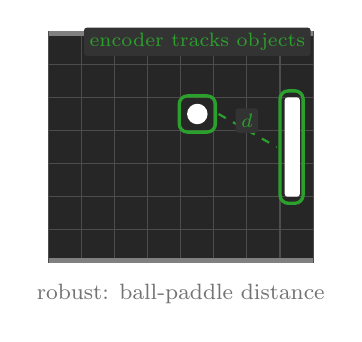
\begin{tikzpicture}[
    lbl/.style={font=\footnotesize, text=black!55},
]
\def\c{0.42}
\def\gw{8}
\def\gh{7}

% Dark game background
\fill[black!85] (0, 0) rectangle ({\gw*\c}, {\gh*\c});
% Subtle grid lines
\foreach \x in {0,...,8} {
    \draw[black!70] (\x*\c, 0) -- (\x*\c, {\gh*\c});
}
\foreach \y in {0,...,7} {
    \draw[black!70] (0, \y*\c) -- ({\gw*\c}, \y*\c);
}

% Top and bottom walls
\fill[black!50] (0, 0) rectangle ({\gw*\c}, {0.15*\c});
\fill[black!50] (0, {6.85*\c}) rectangle ({\gw*\c}, {\gh*\c});

% Paddle
\fill[white!90, rounded corners=1pt]
    ({7*\c + 0.06}, {2*\c}) rectangle ({7.6*\c}, {5*\c});

% Ball
\fill[white] ({4.5*\c}, {4.5*\c}) circle (0.13);

% Green highlight around ball
\draw[palC, very thick, rounded corners=3pt]
    ({4*\c - 0.02}, {4*\c - 0.02})
    rectangle ({5*\c + 0.02}, {5*\c + 0.02});

% Green highlight around paddle
\draw[palC, very thick, rounded corners=3pt]
    ({7*\c}, {1.8*\c})
    rectangle ({7.7*\c}, {5.2*\c});

% Distance line connecting ball to paddle
\draw[palC, thick, dashed]
    ({5*\c + 0.06}, {4.5*\c}) -- ({7*\c - 0.04}, {3.5*\c});
\node[font=\scriptsize, text=palC, fill=black!80,
      inner sep=2pt, rounded corners=1pt]
    at ({6*\c}, {4.3*\c}) {$d$};

% Label
\node[font=\scriptsize, text=palC, fill=black!80,
      inner sep=2pt, rounded corners=1pt, anchor=south]
    at ({4.5*\c}, {6*\c + 0.1})
    {encoder tracks objects};

% Verdict
\node[lbl] at ({4*\c}, {-0.4})
    {robust: ball-paddle distance};

\end{tikzpicture}
\subcaption{The encoder tracks the spatial relationship between
  ball and paddle -- a feature that survives any shift.}
\label{fig:robust-feature}
\end{subfigure}

\caption{Augmentation as regularization. (a)~Without augmentation,
  the encoder can rely on fixed pixel positions.
  (b)~Random shifts force it to learn object relationships.}
\label{fig:fragile-vs-robust}
\end{figure}


\smallskip
Random shift augmentation addresses this directly. Each time a
transition is replayed, the observation is augmented with a
different random spatial shift. Even though the buffer contains
only 100{,}000 transitions, the network never sees the exact same
input twice. This effectively expands the training distribution:
each transition generates a family of slightly different training
examples, all sharing the same Q-value target because the game
semantics are unchanged. The encoder is forced to learn features
that are invariant to small spatial shifts -- features that capture
``where the paddle is relative to the ball'' rather than ``what
pixel values appear at specific coordinates.'' This is
\emph{implicit regularization}: not an explicit penalty in the loss
function, but a constraint on what the encoder can learn, imposed
by the data distribution it trains on.

\smallskip
The same mechanism explains why augmentation helps in supervised
learning: random crops force a classifier to recognize objects
regardless of their position in the frame. In RL, the effect is
amplified because the dataset is orders of magnitude smaller --
100{,}000 transitions versus millions of labeled images -- and
because the training distribution shifts as the policy improves,
compounding the risk of overfitting to early, unrepresentative
data.

\smallskip
CURL~\citep{laskin2020curl} combined contrastive learning with
random crop augmentation on data-efficient Rainbow, reporting
improved performance on Atari-100K. The contrastive loss requires
augmentation to generate positive pairs: two different random crops
of the same observation form a positive pair, while crops of
different observations form negative pairs. Because augmentation is
integral to the contrastive objective, the original results could
not distinguish whether the gains came from contrastive learning or
from the augmentation itself. DrQ and RAD answered this question:
augmentation alone, without any contrastive or self-supervised
loss, achieves similar or better results. The augmentation was
doing most of the work. This finding is important for experimental
design: augmentation and representation learning can be studied as
independent factors only when the representation learning method
does not depend on augmentation for its training signal.

\smallskip
Augmentation ensures the encoder sees diverse views of each
observation, encouraging spatial invariance and reducing
overfitting. But it does not change what the encoder is
\emph{trained to predict}. The Q-learning loss remains the sole
objective shaping the encoder's representations, and in the 100K
regime this signal is weak -- targets are bootstrapped from poor
estimates early in training, providing noisy guidance about what
features matter. The encoder may settle on representations that
satisfy the current Q-targets but fail to support further learning.
This is the gap that self-supervised representation learning
addresses: an auxiliary training objective that shapes the
encoder's representations to capture dynamics and structure beyond
what the Q-learning loss alone requires.

\subsection{Target Networks}
\label{subsec:target-networks-bg}

Experience replay solves the data correlation problem, but a second
instability remains. Recall from \cref{subsec:func-approx} that the
TD target in the semi-gradient update depends on the same parameters
$\mathbf{w}$ that are being updated: the target
$R_{t+1} + \gamma \max_a Q(S_{t+1}, a;\, \mathbf{w})$ shifts every
time the network takes a gradient step. The agent is optimizing
toward a goal that moves with every update.

\smallskip
In supervised learning, labels are fixed -- the loss landscape does
not change during training, and SGD can make steady progress toward
a minimum. In Q-learning with function approximation, the
``labels'' are the TD targets, and they depend on the current
parameters. Every step that improves the prediction also shifts the
target, creating a feedback loop: the network's estimates and its
targets chase each other, and training can oscillate or diverge
rather than converge. This is the bootstrapping element of the
deadly triad -- the target depends on the very estimate being
refined.

\smallskip
The solution is to decouple the prediction from the target by
maintaining two copies of the network. The \emph{online network},
with parameters~$\boldsymbol{\theta}$, is the network being
trained -- it receives gradient updates at every step. The
\emph{target network}, with parameters~$\boldsymbol{\theta}^-$, is
a frozen copy used only to compute the TD target. The target
becomes:
%
\[
R_{t+1} + \gamma \max_{a} Q(S_{t+1}, a;\,
  \boldsymbol{\theta}^-),
\]
%
where $\boldsymbol{\theta}^-$ does not change during training.
Because the target is fixed, the loss landscape is stationary and
SGD can make progress toward a stable objective -- the same
conditions that make supervised learning work.

\smallskip
Periodically -- every $C$ gradient steps -- the target network is
replaced with a copy of the online network:
$\boldsymbol{\theta}^- \leftarrow \boldsymbol{\theta}$. In the
original DQN, $C = 10{,}000$. Between these updates, the target
network is completely frozen: no gradients flow through it, and its
parameters do not change. \Cref{fig:target-network} illustrates this
asymmetry: gradients update only the online network, while the target
network provides a stable reference.

\begin{figure}[ht]
\centering
% Thesis-wide categorical color palette
% Usage: % Thesis-wide categorical color palette
% Usage: \input{figures/palette} in any figure file
%
% Muted primary colors -- print-friendly, visually distinct.
% Inspired by Cooper Union's red/blue primaries, softened for
% academic figures. Use palA-palC for data series in scatter
% plots, line charts, bar charts, etc.

\definecolor{palA}{HTML}{1F77B4}   % Tableau blue
\definecolor{palB}{HTML}{D62728}   % Tableau red
\definecolor{palC}{HTML}{2CA02C}   % Tableau green
 in any figure file
%
% Muted primary colors -- print-friendly, visually distinct.
% Inspired by Cooper Union's red/blue primaries, softened for
% academic figures. Use palA-palC for data series in scatter
% plots, line charts, bar charts, etc.

\definecolor{palA}{HTML}{1F77B4}   % Tableau blue
\definecolor{palB}{HTML}{D62728}   % Tableau red
\definecolor{palC}{HTML}{2CA02C}   % Tableau green

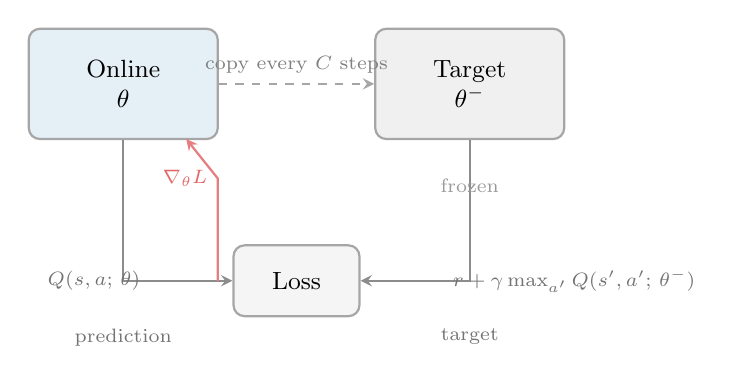
\begin{tikzpicture}[
    net/.style={draw=black!35, thick, rounded corners=4pt,
                minimum width=2.4cm, minimum height=1.4cm,
                font=\small, align=center, inner sep=6pt},
    lossbox/.style={draw=black!35, thick, rounded corners=4pt,
                    minimum width=1.6cm, minimum height=0.9cm,
                    font=\small, fill=black!4},
    arr/.style={->, thick, >=stealth, black!45},
    garr/.style={->, thick, >=stealth, palB!60},
    darr/.style={->, thick, >=stealth, black!35, dashed},
    lbl/.style={font=\scriptsize, text=black!55},
]

% Online network
\node[net, fill=palA!12] (online)
    at (-2.2, 0) {Online\\$\boldsymbol{\theta}$};

% Target network
\node[net, fill=black!6] (target)
    at (2.2, 0) {Target\\$\boldsymbol{\theta}^-$};

% Loss node
\node[lossbox] (loss) at (0, -2.5) {Loss};

% Prediction arrow (online -> loss)
\draw[arr] (online.south) -- (-2.2, -2.5) -- (loss.west)
    node[lbl, pos=0.25, left] {$Q(s, a;\, \boldsymbol{\theta})$};

% Target arrow (target -> loss)
\draw[arr] (target.south) -- (2.2, -2.5) -- (loss.east)
    node[lbl, pos=0.25, right]
    {$r + \gamma \max_{a'} Q(s', a';\, \boldsymbol{\theta}^-)$};

% Gradient arrow (loss -> online)
\draw[garr] (-1.0, -2.5) -- (-1.0, -1.2)
    -- (-1.4, -0.7)
    node[lbl, pos=0.0, left, text=palB!70]
    {$\nabla_{\boldsymbol{\theta}} L$};

% No gradient indicator on target side
\node[font=\scriptsize, text=black!40] at (2.2, -1.3)
    {frozen};

% Copy arrow (online -> target, dashed)
\draw[darr] (online.east) -- (target.west)
    node[lbl, midway, above, text=black!50]
    {copy every $C$ steps};

% Prediction label
\node[lbl, below=1pt] at (-2.2, -2.95)
    {prediction};

% Target label
\node[lbl, below=1pt] at (2.2, -2.95)
    {target};

\end{tikzpicture}
\caption{Target network mechanism. The online network receives
  gradient updates; the target network is frozen and provides stable
  TD targets. Periodically, the online parameters are copied over.}
\label{fig:target-network}
\end{figure}


\smallskip
With both stabilization techniques in place, the complete DQN loss
combines experience replay and the target network:
%
\begin{equation}
\label{eq:dqn-loss}
L(\boldsymbol{\theta}) = \mathbb{E}_{(s,a,r,s') \sim \mathcal{D}}
  \Big[\big(r + \gamma \max_{a'} Q(s', a';\,
  \boldsymbol{\theta}^-) - Q(s, a;\, \boldsymbol{\theta})
  \big)^2\Big].
\end{equation}
%
This is the function approximation loss from \cref{eq:fa-loss} with
two concrete changes. The expectation is over minibatches sampled
uniformly from the replay buffer~$\mathcal{D}$, addressing the data
correlation problem. And the target uses frozen
parameters~$\boldsymbol{\theta}^-$ instead of the current
parameters~$\boldsymbol{\theta}$, stabilizing the optimization
target. These two changes -- replay and frozen targets -- are DQN's
core algorithmic contribution, and they are what make Q-learning
with a deep neural network stable enough to
learn~\citep{mnih2015human}.

\smallskip
The update interval $C$ controls a trade-off between stability and
staleness. A longer interval gives more stability -- the target
moves less frequently, and SGD has more time to converge toward it.
But it also makes the target more stale, since
$\boldsymbol{\theta}^-$ falls further behind
$\boldsymbol{\theta}$ as training progresses. Too long, and the
agent trains against an outdated target that no longer reflects its
current knowledge; too short, and the target moves so often that the
stability benefit is lost.

\smallskip
Together, experience replay and target networks address two of the
three instabilities in the deadly triad: correlated training data
and a shifting optimization target. They do not eliminate the third
element -- the use of a nonlinear function approximator -- but they
reduce the practical instability enough for learning to succeed.
The next section introduces Rainbow, which extends DQN with six
additional improvements that further boost performance.

\subsection{Rainbow Extensions}
\label{subsec:rainbow-extensions}

Between 2015 and 2018, several independent lines of research each
identified a specific weakness in DQN and proposed a targeted fix.
\citet{hessel2018rainbow} showed that combining six of these
improvements into a single agent -- \emph{Rainbow} -- produces
performance far exceeding any individual extension. The gains are
largely complementary, not redundant: each improvement addresses a
different aspect of learning, and their benefits compound when used
together. \Cref{tab:rainbow-extensions} summarizes the six
extensions; the paragraphs below describe each one.

\begin{table}[ht]
\centering
\renewcommand{\arraystretch}{1.4}
\begin{tabular}{lll}
\toprule
Extension & DQN Component Modified & Key Change \\
\midrule
Double DQN       & Target computation
    & Decouple action selection from evaluation \\
Prioritized replay & Replay sampling
    & Weight transitions by TD error \\
Dueling networks & Network head
    & Separate value and advantage streams \\
Multi-step returns & Target computation
    & Bootstrap after $n$ steps, not one \\
Distributional RL  & Loss function
    & Model return distribution, not mean \\
Noisy networks   & Exploration
    & Learned noise replaces $\varepsilon$-greedy \\
\bottomrule
\end{tabular}
\caption{Rainbow's six extensions to DQN. Each targets a different
  component; the convolutional encoder is unchanged.}
\label{tab:rainbow-extensions}
\end{table}


\smallskip
\textbf{Double DQN.}\quad The $\max$ operator in the Q-learning
target (\cref{eq:dqn-loss}) causes a systematic upward bias: when
Q-value estimates are noisy, taking the maximum over noisy values
tends to select overestimates. To see why, imagine four actions
whose true Q-values are all $5.0$, but the noisy estimates are
$4.8$, $5.3$, $4.7$, and $5.1$. The max picks $5.3$,
overestimating the true maximum of $5.0$. The noise is symmetric --
some estimates are too high, some too low -- but the max operator
always selects the highest error. Double
DQN~\citep{van2016deep} fixes this by decoupling action
selection from action evaluation. The online network selects the
best action, but the target network evaluates it -- reducing the
overestimation because two independent estimates are unlikely to
both be biased in the same direction for the same action.

\smallskip
\textbf{Prioritized experience replay.}\quad Standard experience
replay samples transitions uniformly from the buffer, but not all
transitions are equally informative. Prioritized
replay~\citep{schaul2016prioritized} samples transitions with
probability proportional to their TD error -- the magnitude of the
difference between the predicted and target Q-values. Transitions
where the agent's prediction was furthest off are replayed more
often, focusing learning on the most surprising or informative
experiences. Non-uniform sampling introduces a bias, however: the
gradient is weighted toward high-priority transitions, distorting
the loss landscape. Importance sampling weights correct this by
down-weighting transitions that are sampled more frequently than
they would be under uniform sampling. The correction strength is
controlled by a parameter~$\beta$ that increases during training,
gradually shifting from a partial correction toward full correction.

\smallskip
\textbf{Dueling networks.}\quad Rather than estimating $Q(s, a)$
directly, the dueling architecture~\citep{wang2016dueling}
decomposes the Q-value into a state-value $V(s)$ and an advantage
$A(s, a)$, combining them as
$Q(s, a) = V(s) + A(s, a) - \overline{A}(s)$. Both streams share
the convolutional encoder but have separate fully connected heads.
This separation lets the network learn ``how good is this state''
independently from ``how much better is this action than average,''
which is beneficial in states where the choice of action matters
little. In Pong, when the ball is far away, all actions have
roughly equal value -- the important thing is whether the state
itself is safe or dangerous, which the value stream captures.
When the ball is close and the paddle must move, one action is
clearly better, and the advantage stream activates. By separating
these two judgments, the network can learn ``this is a good state''
without needing to differentiate actions in states where the
difference is small. \Cref{fig:dueling-architecture} contrasts the
two architectures.

\begin{figure}[ht]
\centering
% Thesis-wide categorical color palette
% Usage: % Thesis-wide categorical color palette
% Usage: \input{figures/palette} in any figure file
%
% Muted primary colors -- print-friendly, visually distinct.
% Inspired by Cooper Union's red/blue primaries, softened for
% academic figures. Use palA-palC for data series in scatter
% plots, line charts, bar charts, etc.

\definecolor{palA}{HTML}{1F77B4}   % Tableau blue
\definecolor{palB}{HTML}{D62728}   % Tableau red
\definecolor{palC}{HTML}{2CA02C}   % Tableau green
 in any figure file
%
% Muted primary colors -- print-friendly, visually distinct.
% Inspired by Cooper Union's red/blue primaries, softened for
% academic figures. Use palA-palC for data series in scatter
% plots, line charts, bar charts, etc.

\definecolor{palA}{HTML}{1F77B4}   % Tableau blue
\definecolor{palB}{HTML}{D62728}   % Tableau red
\definecolor{palC}{HTML}{2CA02C}   % Tableau green

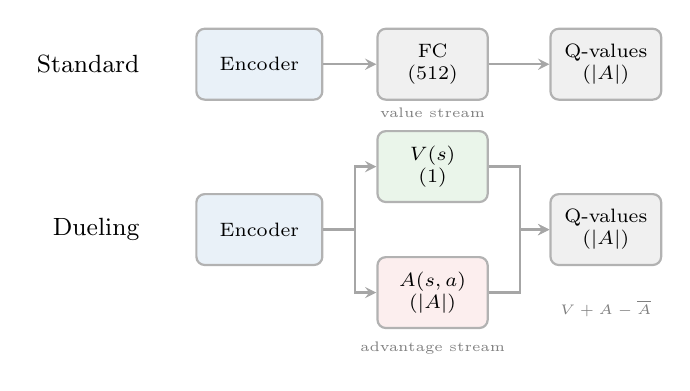
\begin{tikzpicture}[
    block/.style={draw=black!30, thick, rounded corners=3pt,
                  minimum height=0.9cm, font=\scriptsize,
                  align=center, inner sep=5pt},
    arr/.style={->, thick, >=stealth, black!35},
    lbl/.style={font=\tiny, text=black!50},
]

% --- Standard DQN (top) ---
\node[font=\small, anchor=east] at (-0.6, 1.8) {Standard};

\node[block, fill=palA!10, minimum width=1.6cm]
    (enc1) at (0.8, 1.8) {Encoder};
\node[block, fill=black!6, minimum width=1.4cm]
    (fc1) at (3.0, 1.8) {FC\\(512)};
\node[block, fill=black!6, minimum width=1.4cm]
    (q1) at (5.2, 1.8) {Q-values\\($|A|$)};

\draw[arr] (enc1) -- (fc1);
\draw[arr] (fc1) -- (q1);

% --- Dueling (bottom) ---
\node[font=\small, anchor=east] at (-0.6, -0.3) {Dueling};

\node[block, fill=palA!10, minimum width=1.6cm]
    (enc2) at (0.8, -0.3) {Encoder};

% Value stream
\node[block, fill=palC!10, minimum width=1.4cm]
    (v) at (3.0, 0.5) {$V(s)$\\(1)};

% Advantage stream
\node[block, fill=palB!8, minimum width=1.4cm]
    (a) at (3.0, -1.1) {$A(s, a)$\\($|A|$)};

% Combine
\node[block, fill=black!6, minimum width=1.4cm]
    (q2) at (5.2, -0.3) {Q-values\\($|A|$)};

\draw[arr] (enc2.east) -- ++(0.4, 0) |- (v.west);
\draw[arr] (enc2.east) -- ++(0.4, 0) |- (a.west);
\draw[arr] (v.east) -- ++(0.4, 0) |- (q2.west);
\draw[arr] (a.east) -- ++(0.4, 0) |- (q2.west);

% Stream labels
\node[lbl, above=1pt] at (v.north) {value stream};
\node[lbl, below=1pt] at (a.south) {advantage stream};

% Combine label
\node[lbl] at (5.2, -1.3)
    {$V + A - \overline{A}$};

\end{tikzpicture}
\caption{Dueling architecture. The encoder output splits into a
  value stream $V(s)$ and an advantage stream $A(s, a)$, which
  recombine to produce Q-values.}
\label{fig:dueling-architecture}
\end{figure}


\smallskip
\textbf{Multi-step returns.}\quad Standard DQN bootstraps from the
immediate next state -- a one-step target. Multi-step
returns~\citep{sutton2018reinforcement} instead use the actual
rewards from the next $n$ steps before bootstrapping, computing the
target as
$\sum_{k=0}^{n-1} \gamma^k R_{t+k+1}
  + \gamma^n \max_a Q(S_{t+n}, a)$.
This propagates reward information faster and shifts the
bias--variance trade-off: more real rewards and less bootstrapping
reduces bias at the cost of higher variance. The bias reduction
comes from relying less on the bootstrap estimate
$Q(S_{t+n}, a)$, which may be inaccurate early in training: by
substituting real observed rewards for the first~$n$ steps, the
target is grounded in actual experience rather than the network's
current estimates. The variance increase is the cost: real rewards
depend on the specific trajectory the agent happened to take, which
varies from episode to episode. Rainbow uses $n = 3$.

\smallskip
\textbf{Distributional RL.}\quad Instead of estimating the expected
return -- a single number -- distributional
RL~\citep{bellemare2017distributional} models the full distribution
of possible returns. The C51 variant used in Rainbow represents this
distribution as a probability mass function over 51 evenly spaced
values. The network outputs probabilities for each value, and the
loss minimizes the KL divergence -- a measure of how different two
probability distributions are -- between the predicted and target
distributions. Modeling the full distribution provides a richer
training signal than predicting the mean alone: two states might
have the same expected return of $+5$, but very different risk
profiles -- one always yielding $+5$, the other yielding $+10$ or
$0$ with equal probability. The distributional loss forces the
encoder to distinguish these states, even though the policy still
acts on the expected value.
\Cref{fig:distributional-output} illustrates the difference in
output structure.

\begin{figure}[ht]
\centering
% Thesis-wide categorical color palette
% Usage: % Thesis-wide categorical color palette
% Usage: \input{figures/palette} in any figure file
%
% Muted primary colors -- print-friendly, visually distinct.
% Inspired by Cooper Union's red/blue primaries, softened for
% academic figures. Use palA-palC for data series in scatter
% plots, line charts, bar charts, etc.

\definecolor{palA}{HTML}{1F77B4}   % Tableau blue
\definecolor{palB}{HTML}{D62728}   % Tableau red
\definecolor{palC}{HTML}{2CA02C}   % Tableau green
 in any figure file
%
% Muted primary colors -- print-friendly, visually distinct.
% Inspired by Cooper Union's red/blue primaries, softened for
% academic figures. Use palA-palC for data series in scatter
% plots, line charts, bar charts, etc.

\definecolor{palA}{HTML}{1F77B4}   % Tableau blue
\definecolor{palB}{HTML}{D62728}   % Tableau red
\definecolor{palC}{HTML}{2CA02C}   % Tableau green

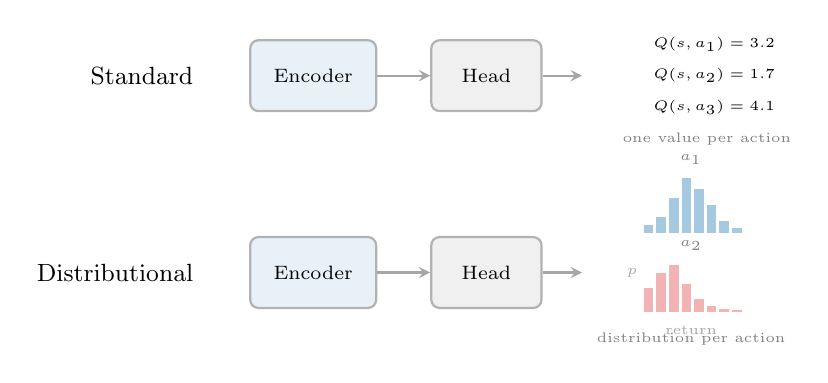
\begin{tikzpicture}[
    block/.style={draw=black!30, thick, rounded corners=3pt,
                  minimum height=0.9cm, font=\scriptsize,
                  align=center, inner sep=5pt},
    arr/.style={->, thick, >=stealth, black!35},
    lbl/.style={font=\tiny, text=black!50},
    bar/.style={thick},
]

% --- Standard DQN (top) ---
\node[font=\small, anchor=east] at (-0.6, 2.0) {Standard};

\node[block, fill=palA!10, minimum width=1.6cm]
    (enc1) at (0.8, 2.0) {Encoder};
\node[block, fill=black!6, minimum width=1.4cm]
    (head1) at (3.0, 2.0) {Head};

\draw[arr] (enc1) -- (head1);

% Scalar Q-values (one per action)
\draw[arr] (head1.east) -- ++(0.5, 0);
\foreach \i/\v in {0/3.2, 1/1.7, 2/4.1} {
    \node[font=\tiny, anchor=west] at (5.0, {2.4 - \i*0.4})
        {$Q(s, a_{\the\numexpr\i+1})=\v$};
}

\node[lbl] at (5.8, 1.2) {one value per action};

% --- Distributional (bottom) ---
\node[font=\small, anchor=east] at (-0.6, -0.5) {Distributional};

\node[block, fill=palA!10, minimum width=1.6cm]
    (enc2) at (0.8, -0.5) {Encoder};
\node[block, fill=black!6, minimum width=1.4cm]
    (head2) at (3.0, -0.5) {Head};

\draw[arr] (enc2) -- (head2);
\draw[arr] (head2.east) -- ++(0.5, 0);

% Distribution for action 1 (small bar chart)
\def\bx{5.0}
\def\by{0.0}
\foreach \i/\h in {0/0.05, 1/0.10, 2/0.22, 3/0.35, 4/0.28,
                    5/0.18, 6/0.08, 7/0.03} {
    \fill[palA!40] ({\bx + \i*0.16}, \by)
        rectangle ({\bx + \i*0.16 + 0.12}, {\by + \h*2.0});
}
\node[lbl, above] at ({\bx + 0.6}, {\by + 0.75}) {$a_1$};

% Distribution for action 2
\def\byy{-1.0}
\foreach \i/\h in {0/0.15, 1/0.25, 2/0.30, 3/0.18, 4/0.08,
                    5/0.04, 6/0.02, 7/0.01} {
    \fill[palB!35] ({\bx + \i*0.16}, \byy)
        rectangle ({\bx + \i*0.16 + 0.12}, {\byy + \h*2.0});
}
\node[lbl, above] at ({\bx + 0.6}, {\byy + 0.65}) {$a_2$};

\node[lbl] at ({\bx + 0.6}, -1.35) {distribution per action};

% Axis labels
\node[font=\tiny, text=black!35] at ({\bx - 0.15}, -0.5)
    {$p$};
\node[font=\tiny, text=black!35, anchor=north]
    at ({\bx + 0.6}, {-1.05}) {return};

\end{tikzpicture}
\caption{Distributional RL output. Standard DQN outputs one scalar
  Q-value per action; C51 outputs a probability distribution over
  possible returns for each action.}
\label{fig:distributional-output}
\end{figure}


\smallskip
\textbf{Noisy networks.}\quad DQN uses $\varepsilon$-greedy
exploration, which selects random actions with fixed
probability~$\varepsilon$ regardless of the agent's uncertainty.
Noisy networks~\citep{fortunato2018noisy} replace this with learned
parametric noise injected into the network's weights. The network
learns to explore where it is uncertain and exploit where it is
confident, rather than exploring uniformly at random. With noisy
networks, $\varepsilon$ is set to zero -- action selection is fully
greedy with respect to the (noisy) Q-values.

\subsection{The Rainbow Agent}
\label{subsec:rainbow-agent}

Taken together, these six extensions modify nearly every component
of DQN: the loss function changes from squared error to
distributional KL divergence, the replay strategy from uniform to
prioritized sampling, the target computation from single-step to
multi-step with double Q-learning, the exploration strategy from
$\varepsilon$-greedy to noisy networks, and the network head from
a single stream to the dueling architecture. The only component
left unchanged is the convolutional encoder -- the Nature CNN
backbone from \cref{subsec:dqn-architecture}.
\Cref{fig:rainbow-components} maps each extension to the component
it modifies, highlighting the encoder as the sole unchanged piece.

\begin{figure}[ht]
\centering
% Thesis-wide categorical color palette
% Usage: % Thesis-wide categorical color palette
% Usage: \input{figures/palette} in any figure file
%
% Muted primary colors -- print-friendly, visually distinct.
% Inspired by Cooper Union's red/blue primaries, softened for
% academic figures. Use palA-palC for data series in scatter
% plots, line charts, bar charts, etc.

\definecolor{palA}{HTML}{1F77B4}   % Tableau blue
\definecolor{palB}{HTML}{D62728}   % Tableau red
\definecolor{palC}{HTML}{2CA02C}   % Tableau green
 in any figure file
%
% Muted primary colors -- print-friendly, visually distinct.
% Inspired by Cooper Union's red/blue primaries, softened for
% academic figures. Use palA-palC for data series in scatter
% plots, line charts, bar charts, etc.

\definecolor{palA}{HTML}{1F77B4}   % Tableau blue
\definecolor{palB}{HTML}{D62728}   % Tableau red
\definecolor{palC}{HTML}{2CA02C}   % Tableau green

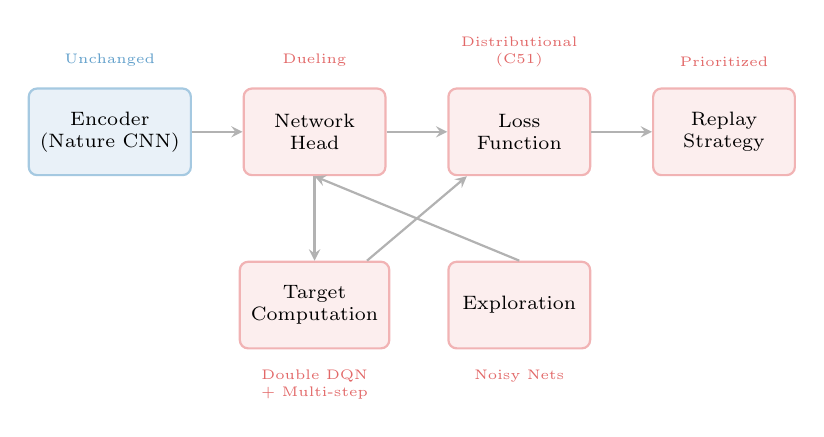
\begin{tikzpicture}[
    comp/.style={draw=black!30, thick, rounded corners=3pt,
                 minimum width=1.8cm, minimum height=1.1cm,
                 font=\scriptsize, align=center, inner sep=4pt},
    unchanged/.style={comp, fill=palA!10, draw=palA!40},
    changed/.style={comp, fill=palB!8, draw=palB!35},
    arr/.style={->, thick, >=stealth, black!30},
    ext/.style={font=\tiny, text=palB!70, align=center},
    ulbl/.style={font=\tiny, text=palA!70},
]

% Components (left to right flow)
\node[unchanged] (enc) at (0, 0) {Encoder\\(Nature CNN)};
\node[changed]   (head) at (2.6, 0) {Network\\Head};
\node[changed]   (loss) at (5.2, 0) {Loss\\Function};
\node[changed]   (replay) at (7.8, 0) {Replay\\Strategy};

% Second row
\node[changed]   (target) at (2.6, -2.2) {Target\\Computation};
\node[changed]   (explore) at (5.2, -2.2) {Exploration};

% Arrows
\draw[arr] (enc) -- (head);
\draw[arr] (head) -- (loss);
\draw[arr] (loss) -- (replay);
\draw[arr] (head) -- (target);
\draw[arr] (target) -- (loss);
\draw[arr] (explore.north) -- (head.south);

% Extension labels
\node[ext, above=4pt] at (head.north)  {Dueling};
\node[ext, above=4pt] at (loss.north)  {Distributional\\(C51)};
\node[ext, above=4pt] at (replay.north) {Prioritized};
\node[ext, below=4pt] at (target.south)
    {Double DQN\\+ Multi-step};
\node[ext, below=4pt] at (explore.south) {Noisy Nets};

% Unchanged label
\node[ulbl, above=4pt] at (enc.north) {Unchanged};

\end{tikzpicture}
\caption{Rainbow modifies five of six DQN components. The
  convolutional encoder -- where SPR operates -- is the only
  component left unchanged.}
\label{fig:rainbow-components}
\end{figure}


\smallskip
\citet{hessel2018rainbow} performed ablation experiments, removing
one component at a time to measure each extension's contribution.
The most critical components were prioritized replay and multi-step
returns; the least impactful in isolation were double Q-learning and
dueling networks. However, this ranking was established at 200
million frames of training. Whether the same ranking holds in the
data-efficient regime -- where the agent has far fewer interactions
to learn from -- is less clear, as the relative importance of each
component may shift when data is scarce.

\smallskip
That the convolutional encoder remains unchanged across all of these
improvements is significant. Methods such as SPR, introduced in
\cref{subsec:spr}, add self-supervised objectives that operate
directly on the encoder's learned representations. When SPR was
shown to improve Rainbow's performance, it was unclear whether the
gains came from SPR's representation learning or from Rainbow's many
enhancements providing a richer learning substrate. Disentangling
these factors -- testing whether SPR's benefits transfer to a
simpler base agent -- is one of the questions that motivates the
experiments in this work.
